\chapter{Reconstruction, Cleaning and Analysis Techniques}
\label{ch:reconstruction}
\begin{flushright}
\textit{Shall I refuse my dinner because I do not fully understand the process of digestion? $\sim$ Oliver Heaviside}
\end{flushright}
As explained in Chapter \ref{ch:icecube}, an IceCube event consists of a series of DOM hits. One hit contains charge, timing, and positional information. This collection of multiple hits has to be translated (reconstructed) to certain properties of a particle. Some examples are the direction, position, track length, etc. Fast reconstructions of these properties, such as the ones necessary in online filtering, are usually done with simple algorithms. More sophisticated algorithms are performed offline on smaller data samples.\\

\noindent Because the in-ice IceCube detector is sparsely distributed, it is not straightforward to unambiguously reconstruct the particle (interactions). The scattering and absorption of photons, tilt of ice sheets, bubble columns, etc. lead to uncertainties and make reconstruction challenging. Over the years, multiple different methods have been developed in the collaboration. Several reconstruction algorithms have been used in this analysis and are explained in more detail in this chapter. We start with the algorithms that reconstruct where the particle entered and in which direction it traversed the detector and give an estimate on the direction uncertainty.

A number of hits in an event can often be attributed to DOM noise. There are several techniques possible to remove these hits, some of which are used in this analysis. They are also discussed in more detail below.

Finally, we discuss the methods that were used to discriminate signal from background events with machine learning techniques.

\section{Reconstruction}

\subsection{Likelihood}
Reconstruction algorithms usually have no unique solutions to describe the set of measured values of an event. The likelihood $\mathcal{L}(\vec{x} |\vec{a})$ describes the probability of a set of parameters ${\vec{a}}$ to be expressed in a set of experimentally measured values ${\vec{x}}$. The parameters, ${\vec{a}}$, typically define the particle's characteristics (energy, direction, position, type, etc.) while the measured values ${\vec{x}}$ are determined from the detector response (number of PE, timing, position of hit DOMs, etc.). This likelihood is equal to the cumulative probability

\begin{equation}
\mathcal{L}(\vec{x}|\vec{a}) = \prod_i p(x_i|\vec{a}),
\end{equation}
\noindent where $p(x,\vec{a})$ is the probability that we measure a certain value $x$ from a set of independent values $\vec{x}$, given an initial set of parameters $\vec{a}$. The maximum likelihood method is used to estimate the unknown parameters $\vec{a}$, which is done by maximizing $\mathcal{L}$. The reconstruction algorithms below rely on analyzing parameters that assume a single, long track

\begin{equation}
\label{eq:vec}
\vec{a} = (\vec{r_0},t_0,\hat{\vec{p}},E_0),
\end{equation}
\noindent where $\vec{r_0}$ is the position vector of the particle at a time $t_0$ with a direction $\hat{\vec{p}}$ and initial energy $E_0$. 

\subsection{\texttt{Line-Fit}}
\label{subsec:lf}

\begin{figure}
\centering
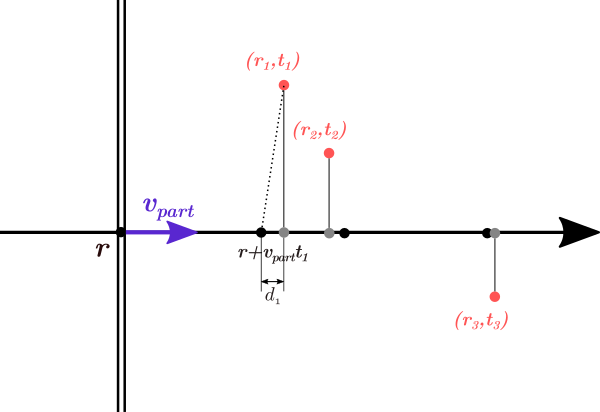
\includegraphics[width=0.6\textwidth]{chapter7/img/linefit2.png}
\caption{Figure illustrating how \texttt{LineFit} works. The position, $\vec{r}$, and velocity, $\vec{v}_\textrm{part}$ minimizing the distance of the DOMs to the track is calculated. The dotted line is one of the distances that is minimized in Eq. \ref{eq:lf}.}
\label{fig:lf}
\end{figure}

\noindent One of the simplest approaches in constructing a parameter profile is by calculating the track that, overall, has the closest approach of all the hit optical modules. This is called \texttt{Line-Fit}\index{Line-Fit} (LF) \cite{Ahrens:2003fg}. If we assume that a particle starts at a position $\vec{r}$ at a time $t=0$ and travels at a velocity of $\vec{v}_\textrm{part}$, then its position at any given time is

\begin{equation}
\vec{r'} = \vec{r} + \vec{v}_{\textrm{part}}t.
\end{equation}

\noindent We want to calculate the best possible estimate of the velocity $\vec{v}_\textrm{part}$ and an initial position $\vec{r}$. Each DOM has a known location, $\vec{r}_i$, and measured time of a pulse, $t_i$. In this algorithm, one assumes that a wavefront perpendicular to the particle's direction is traveling along with the particle. If the velocity $\vec{v}_\textrm{part}$ is fixed, then the position of the particle at later times is known (black points in Figure \ref{fig:lf}). However, the Cherenkov wavefront should be set at an angle and because scattering, PMT jitter, noise, etc. are not taken into account, this will not agree with the DOM position projected along the particle path (grey dots). The unknown velocity $\vec{v}_\textrm{part}$ and position $\vec{r}$ are the analytical solutions after minimizing the distances $d_i$ as shown in the figure\footnote{Minimizing $r_i - r'$ (dotted line in Figure \ref{fig:lf}) is the same as minimizing $d$.}

\begin{equation}
\label{eq:lf}
\begin{split}
S(\vec{r},\vec{v}_{\textrm{part}}) &\equiv \sum^{N_{\textrm{hit}}}_{i=1} \rho^2(\vec{r},\vec{v}_\textrm{part},\vec{r}_i,t_i)\\
&= \sum^{N_{\textrm{hit}}}_{i=1} \left(\vec{r}_i - \vec{r} - \vec{v}_\textrm{part}t_i \right)^2,
\end{split}
\end{equation}
\noindent where $\rho(\vec{r},\vec{v}_\textrm{part},\vec{r}_i,t_i) = \left|\vec{r}_i - \vec{r} - \vec{v}_\textrm{part}t_i \right|$ and $N_\textrm{hit}$ is the number of pulse hits. The analytical solution by minimizing this equation is equal to

\begin{equation}
\vec{r} = \langle\vec{r}_i\rangle - \vec{v}_\textrm{part}\langle t_i\rangle \ \ \ \textrm{and}\ \ \ \vec{v}_\textrm{part} = \frac{\langle \vec{r}_i t_i\rangle - \langle \vec{r}_i \rangle \langle t_i \rangle }{\langle t_i^2 \rangle - \langle t_i \rangle^2},
\end{equation}
\noindent where $\langle x \rangle$ denotes the average of a parameter $x$ over all hits $i$.

Because this is an analytical equation, this algorithm is very fast and is therefore often used in online processing.
 
\subsubsection{\texttt{Improved Line-Fit}}
\texttt{Line-Fit} is usually implemented as a seed track for other, more computationally heavy algorithms (such as SPE, see Section \ref{subsec:spempe}). The simplifications that are used in LF can lead to angular deviations that converge to a local minimum instead of the global. The LF algorithm assumes that all hits will be near the track and hits far away from the track enter the least squares computation quadratically. Therefore, hits from far away often dominate the reconstruction even though the simple algorithm doesn't account for 

\vspace{2mm}
\begin{enumerate}
\item The Cherenkov emission profile.
\item The scattering effects of the ice medium.
\item Noise hits that occur far from the track.
\end{enumerate}
\vspace{2mm}

\noindent To reduce the effects of outliers, it was found that a basic filter could identify these scattered hits, and improve accuracy by almost a factor of two by removing them from the dataset. More formally, for each hit $h_i$ (that consists of a charge, position and timing), the algorithm looks at all neighboring hits within a neighborhood of radius $\mu$, and if there exists a neighboring hit $h_j$ with a time stamp that is $t$ earlier than $h_i$, then $h_i$ is considered a scattered hit and is not used in the basic reconstruction algorithm. Optimal values of $\mu$ and $t$ were found to be 156 m and 778 ns by tuning them on simulated muon data \cite{Aartsen:2013bfa}.\\

\noindent This ``delay cleaning'' is done by computing a Huberfit on the remaining data points and minimizing

\begin{equation}
\sum^{N_{\textrm{hit}}}_{i=1} \phi(\rho(\vec{r},\vec{v}_\textrm{part},\vec{r}_i,t_i)),
\end{equation}
\noindent where $\rho$ is defined in Eq. \ref{eq:lf} and the Huber penalty function $\phi$ is defined as

\begin{equation}
\phi(\rho) \equiv \left\{
    \begin{array}{ll}
        \rho^2 &\textrm{if } \rho < \mu \\
        \mu\left(2\rho - \mu\right) & \textrm{if }\rho \geq \mu
    \end{array}
    \right.
    .
\end{equation}
\noindent An example of the Huber penalty function is given in Figure \ref{fig:huberpenalty}. Because of the overall performance increase of this method, all LF computations were done with the improved version (although still often referred to as ``Line-Fit'').

\begin{figure}
\centering
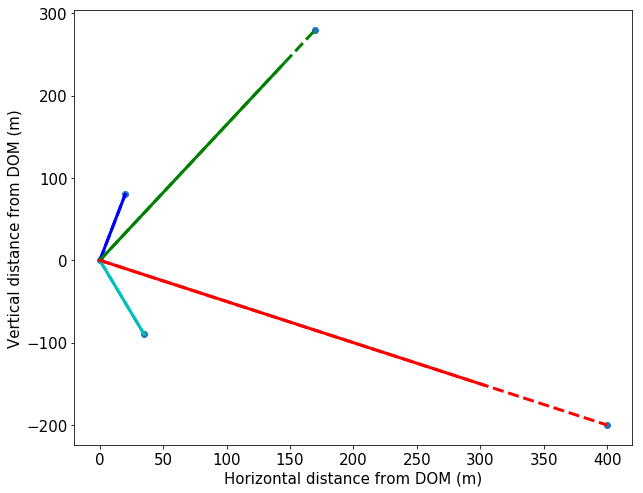
\includegraphics[width=0.7\textwidth]{chapter7/img/exampleHuber.png}
\caption{Illustration of Huber penalty for possible hit locations. The origin was set as the assumed particle position, $\vec{r}+\vec{v}_\textrm{part}t_i$. The solid line shows the result of $\phi(\rho)$ where the dotted lines show values for $\rho$.}
\label{fig:huberpenalty}
\end{figure}

\subsection{SPE and MPE}
\label{subsec:spempe}
A more intricate method of track reconstruction is done by taking the geometrical shape of the Cherenkov cone into account and relying on simulation fits where a seed track is implemented (usually from the fast \texttt{Line-Fit} algorithm) \cite{Ahrens:2003fg}.


\begin{figure}
\centering
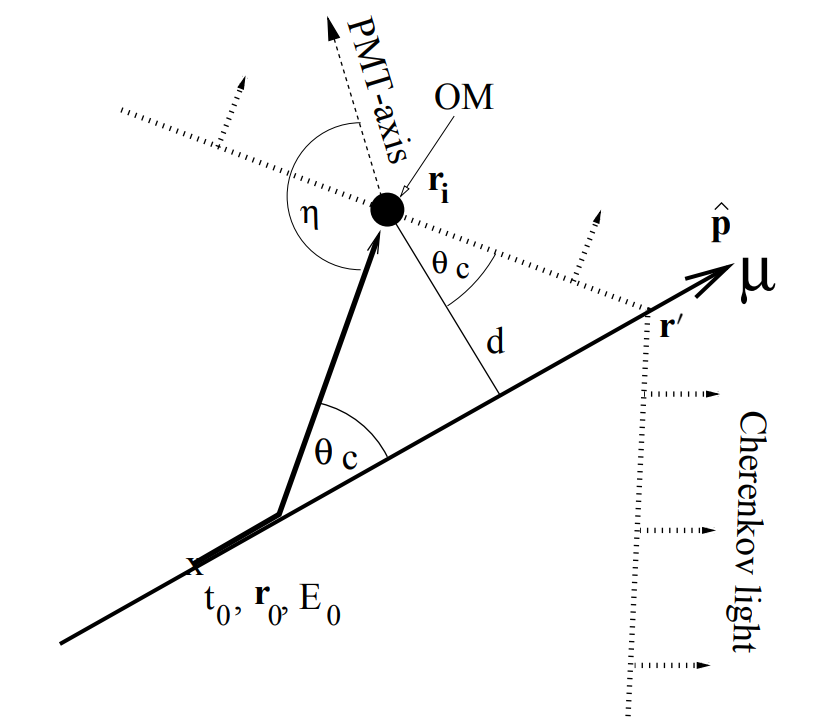
\includegraphics[width=0.6\textwidth]{chapter7/img/reconstruction.png}
\caption{Figure illustrating a muon track passing close by an optical module and defining the parameters used in the reconstruction algorithms. Illustration from Ref. \cite{Ahrens:2003fg}.}
\label{fig:reconstruction}
\end{figure}

Let us assume a particle is traveling close to a DOM with parameters as defined in Eq. \ref{eq:vec} as illustrated in Figure \ref{fig:reconstruction}. The minimal distance of the track to the DOM is equal to $d$ and the PMT-axis (downwards relative to DOM) has an angle offset of $\eta$ degrees of the Cherenkov wave direction. If Cherenkov photons would travel undelayed directly from the primary particle to an OM, the \textit{time residual} (time between the observed hit time and the ``expected'' time) is a delta function centered around 0, where

\begin{equation}
t_{\textrm{res}} \equiv t_{\textrm{hit}} - t_{\textrm{geo}},
\end{equation}
\noindent with

\begin{equation}
t_\textrm{geo} = t_0 + \frac{\hat{\vec{p}} \cdot (\vec{r}_i - \vec{r}_0) + d\cdot \tan (\theta_c)}{c_\textrm{vac}},
\end{equation}
\noindent which is the time necessary for the particle to travel from the position $\vec{r}_0$ to $\vec{r}'$ as illustrated in the figure. The accompanying Cherenkov wavefront that sent out photons at a time $t_0$ from $\vec{r}_0$ will cross the DOM when the particle is at a position $\vec{r}'$. Due to noise effects, PMT jitter, light from secondary interactions, DOM orientation, etc. the time residual is smeared and shifted as can be seen in Figure \ref{fig:spempejitter}. Stochastic energy deposits along the track of a high-energy particle (as described in Section \ref{subsub:energyloss}) lead to an additional shift of the time residual since these photons arrive after the Cherenkov cone.

A time likelihood function $\mathcal{L}_\textrm{time}$ can be constructed from the p.d.f. of arrival times of single photons, $p_1$, at the locations of the hit DOMs. The p.d.f. of single photons was estimated with photon simulations in ice and fitted to a \textit{Pandel function}. How this was done and for more information on this function, I refer the reader to Ref. \cite{Ahrens:2003fg}. 

\begin{figure}[t]
\centering
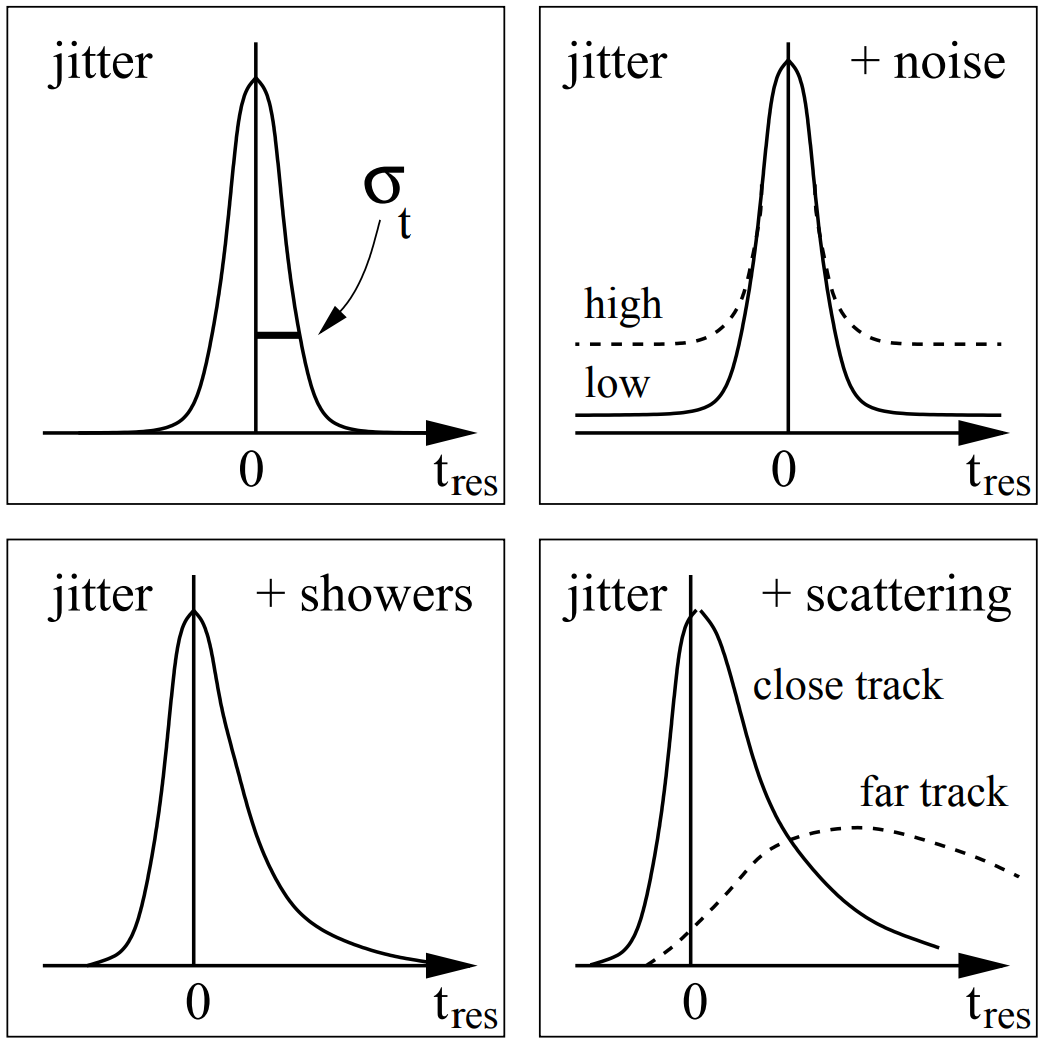
\includegraphics[width=0.5\textwidth]{chapter7/img/spempejitter.png}
\caption{Schematic distributions of $t_\textrm{res}$ where several effects are included. \textit{Top left: }PMT jitter effects. \textit{Top right: }jitter and random noise effects. \textit{Bottom left: }adding indirect Cherenkov light from stochastic deposits along the track of a high-energy particle. \textit{Bottom right: }adding scattering delay effects. Figure from Ref. \cite{Ahrens:2003fg}.}
\label{fig:spempejitter}
\end{figure}

\begin{equation}
\label{eq:spelikelihood}
\mathcal{L}_\textrm{time} = \sum^{N_\textrm{hit}}_{i=1} p_1 (t_\textrm{res} | \vec{a} = {d_i,\eta_i,...}).
\end{equation}
\noindent An initial particle position and direction is found by maximizing the likelihood and iterated a couple of times to find the global maximum instead of a local. This fitting is called the \textit{Single PhotoElectron (SPE)\index{SPE} fit}.\\

\noindent Unfortunately, the description of single photons arriving at the optical modules is not fully correct since electrical and optical signal channels can only resolve multiple photons separated by a few 100 ns and $\approx$10 ns, respectively. Within this time window, only the arrival time of the first pulse is recorded.\\

\noindent In the \textit{Multi-PhotoElectron (MPE) fit}, one accounts for the fact that the early photons in a DOM hit scattered less in the ice. The p.d.f. for the first photon out of a total of $N$ to arrive with a time residual of $t_\textrm{res}$ is

\begin{equation}
p^1_N (t_\textrm{res}) = N \cdot p_1(t_\textrm{res}) \cdot \left(\int^\infty_{t_\textrm{res}} p_1(t) dt \right)^{(N-1)} = N \cdot p_1 (t_\textrm{res}) \cdot (1-P_1 (t_\textrm{res}))^{(N-1)},
\end{equation}
\noindent where $P_1$ is the cumulative distribution of the single photon p.d.f. The MPE likelihood computation is done by replacing $p_1$ in Eq. \ref{eq:spelikelihood} with $p^1_N$.\\

\noindent Several variables that are obtained from these algorithms were used in this analysis. For example, the direction of the reconstructed particle was used to look for upgoing tracks, while the likelihood of the reconstruction was used to remove downgoing muon tracks that were wrongfully reconstructed as upgoing.

\subsection{\texttt{Paraboloid}}
\label{subsec:paraboloid}

In Sections \ref{subsec:lf} and \ref{subsec:spempe}, we discussed how a particle's direction could be estimated with likelihood estimations. The \texttt{Paraboloid} module tries to provide an estimate for the error on this direction. A highly energetic muon event with hundreds of hit DOMs will lead to a much better directional resolution than a dim track where only a handful of DOMs are hit. In general, the likelihood space around the estimated direction is scanned and compared to the likelihood of the initial track estimation. If the likelihood space around the minimum\footnote{Often minimizers are used in likelihood computations, which actually use $-\log \mathcal{L}$.} is relatively flat, there is a larger uncertainty in the directional estimation. With this method, the module also tries to parameterize if the maximum likelihood that is found from the reconstruction algorithms is far from, or close to the global maximum likelihood. The module uses a minimizer and constructs a grid of zenith and azimuth points near the minimum of the negative likelihood. For each point on the grid, it does a three-parameter minimization for the vertex holding the zenith and azimuth constant. The likelihood values for each point on the grid are then fit to a paraboloid (2D parabola) using a $\chi^2$ minimization since the shape of the log-likelihood space near the minimum should have a paraboloid shape. Of importance are the parameters of the corresponding error, which are assumed to correspond to an ellipse for the $1\sigma$ contours.\\

\noindent The module computes the lengths of the semi-major and semi-minor axes of the $1\sigma$ error ellipse $\sigma_1$ and $\sigma_2$\footnote{The confidence intervals $\sigma_\theta$ and $\sigma_\phi$ can be found by rotating the minor and minor axes $\sigma_1$ and $\sigma_2$.}. It was found that the quadratic mean of both uncertainties provides a good single-valued estimate for the angle uncertainty

\begin{equation}
\label{eq:paraboloid}
\sigma_\textrm{para} = \sqrt{\frac{\sigma_1^2 + \sigma_2^2}{2}}.
\end{equation}

\noindent Since $\sigma_1$ and $\sigma_2$ should follow univariate Gaussian distributions, $\sigma_\textrm{para}$ will be the radius parameter in a bivariate distribution. Also, the great circle distance between the MC truth of the signal particle and the reconstruction direction, as calculated by the Vincenty formula, is a two-dimensional distribution. From the Rayleigh distribution, it follows that the mean of this distribution should be equal to $1.177\sigma_\textrm{para}$\footnote{The CDF of the Rayleigh distribution $1-e^{-x^2/2\sigma^2}$ is equal to the containment for a bivariate normal distribution. Implementing $x=1.177\sigma$ yields a factor of 0.5.}. Therefore, if we divide the great circle distance with $\sigma_\textrm{para}$, we should obtain a variable that is distributed with a peak at 1.177 (mean). This variable is called the \textit{paraboloid pull} and should be compared to an energy related variable (here the number of hit DOMs (NCh) is used). In Figure \ref{fig:paraboloidpull}, it is clear that there is an offset that changes in function of the number of hit DOMs. This effect is seen in all analyses and can be explained by multiple factors in Monte Carlo simulations, but mainly stems from our incomplete knowledge and non-perfect simulations of the ice. The energy-dependent correction factor is computed from Monte Carlo events and applied to both data and MC. From the figure, it is clear that the pull is overestimated ($\sigma_\textrm{para}$ is underestimated), meaning the correction will increase the directional uncertainty $\sigma_\textrm{para}$, which is by any means a conservative method.
More information on this algorithm can be found in Ref. \cite{Neunhoffer:2004ha}.


%meaning that the mean should be set to $1.177\sigma$\footnote{The CDF of the Rayleigh distribution $1-e^{-x^2/2\sigma^2}$ is equal to the containment for a bivariate normal distribution. Implementing $x=1.177\sigma$ yields a factor of 0.5.}, with $\sigma$ the scale of the Rayleigh distribution. The variable $\sigma_\textrm{para}$ describes an uncertainty on the direction estimation. But to know if this uncertainty is distributed like described above, one needs to compare the reconstructed direction with the true particle direction. This means, that if we calculate the great circle distance between the MC truth of the signal particle with the reconstruction direction and divide it by $\sigma_\textrm{para}$, the distribution should peak at 1.177 (mean). This variable is called the \textit{paraboloid pull} and should be compared to an energy related variable (here the number of hit DOMs (NCh) is used). In Figure \ref{fig:paraboloidpull}, it is clear that there is an offset that changes in function of the number of hit DOMs. This effect is seen in all analyses and can be explained by multiple factors in Monte Carlo simulations, but mainly stems from our incomplete knowledge and non-perfect simulations of the ice. The correction factor that depends on the energy is computed from Monte Carlo events and applied to both data and MC.

\begin{figure}[t]
\centering
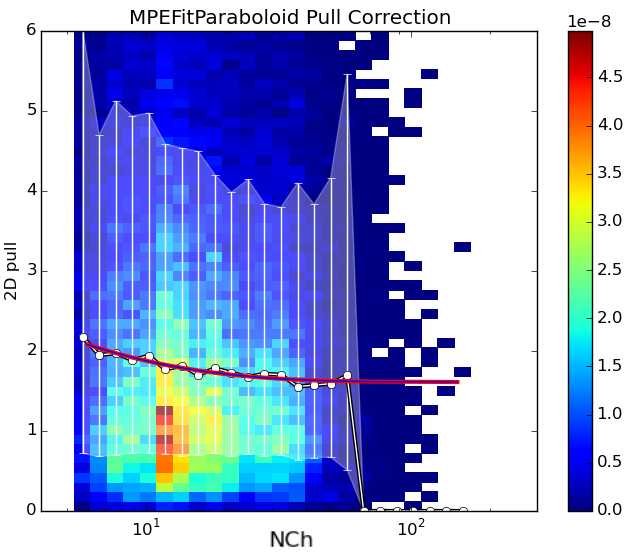
\includegraphics[width=0.48\textwidth]{chapter7/img/pullbeforecorrection.png}
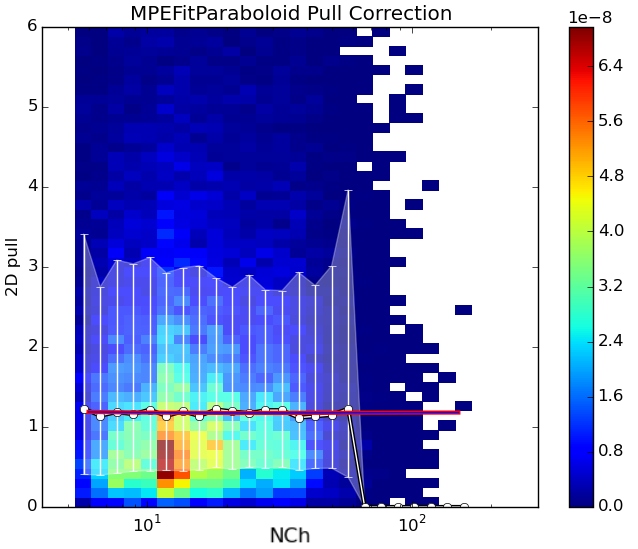
\includegraphics[width=0.48\textwidth]{chapter7/img/pullaftercorrection.png}
\caption{\textit{Left: }Paraboloid pull in function of the number of hit DOMs shows that the global average (red/purple line) is not centered at 1.177. \textit{Right: }Pull after correction.}
\label{fig:paraboloidpull}
\end{figure}

\subsection{\texttt{Millipede}}
\label{subsec:millipede}
To have a better handle on the particle energy and stochastic cascades along the track, the module \texttt{Millipede} was developed \cite{millipedeinternal, Aartsen:2013vja}. The number of photons seen at each optical module depends on multiple factors that were mentioned throughout this text, such as the scattering and absorption in the ice, timing jitter, etc. In this module, the expected number of photons is assumed to depend on the energy that was deposited along a track and a \textit{light yield factor}, $\Lambda$, that depends on the DOM position and the location of emission

\begin{equation}
\label{eq:n_exp}
\begin{split}
N_{\textrm{exp},k} &= \rho_k + \sum^n_{i=1} \Lambda(\vec{r}_k,\vec{r}_i') E_i\\
&= \rho_k + \vec{\Lambda}(\vec{r}_k,\vec{r}_i') \cdot \vec{E},
\end{split}
\end{equation}
where $k$ refers to a certain DOM and $i$ refers to a certain energy deposit such as illustrated in Figure \ref{fig:millipede}. $\rho$ is the average expected number of noise photons and is determined by the duration of the event. The light yield factor and energy are written as vectors to shorten the expressions. 

\begin{figure}
\centering
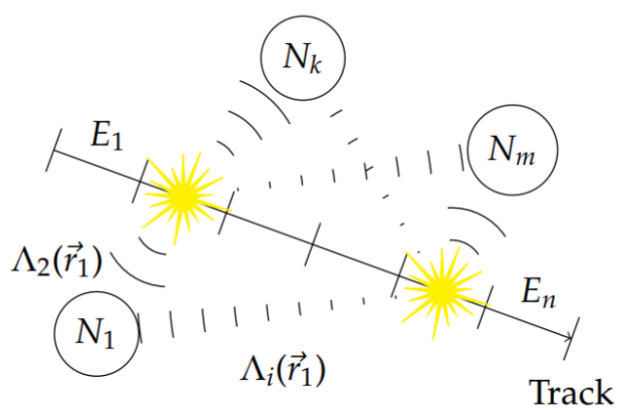
\includegraphics[width=0.6\textwidth]{chapter7/img/millipede.png}
\caption{Illustration of the working principles of the \texttt{Millipede} toolkit. A track is subdivided into segments that each deposit a certain energy, $E_i$. Different segments can contribute to the total number photons seen per DOM, $N_k$.}
\label{fig:millipede}
\end{figure}

The likelihood is assumed to follow a Poisson distribution with $N_{\textrm{seen},k}$ the number of hits that occurred and a mean value equal to the number of expected photons, $N_{\textrm{exp},k}$

\begin{equation}
\begin{split}
\mathcal{L}_k &= \frac{\left(N_{\textrm{exp},k}\right)^{N_\textrm{seen},k}}{N_\textrm{seen},k!} e^{-N_\textrm{exp},k}\\
&= \frac{\left(\vec{\Lambda} \cdot \vec{E} + \rho_k \right)^{N_{\textrm{seen},k}}}{N_{\textrm{seen},k}!} e^{-\vec{\Lambda} \cdot \vec{E} - \rho_k}.
\end{split}
\end{equation}
\noindent For easier, faster and more accurate computation, the logarithm of the likelihood is used

\begin{equation}
\begin{split}
\ln \mathcal{L}_k &= N_{\textrm{seen},k} \ln \left(\rho_k + \sum^n_{i=1} \Lambda(\vec{r}_k,\vec{r}_i') E_i \right) - \ln \left(N_{\textrm{seen},k}!\right) - \sum^n_{i=1} \Lambda(\vec{r}_k,\vec{r}_i') E_i - \rho_k\\
&= N_{\textrm{seen},k} \ln \left(\rho_k + \vec{\Lambda}(\vec{r}_k) \cdot \vec{E} \right) - \vec{\Lambda}(\vec{r}_k) \cdot \vec{E} - \rho_k - \ln\left(N_{\textrm{seen},k}!\right)
\end{split}
\end{equation}
\noindent Assuming a total of $m$ DOMs that registered hits, we can maximize the total likelihood with respect to the energy, which gives 

\begin{equation}
\nabla_{\vec{E}} \ln \mathcal{L} = \nabla_{\vec{E}} \sum^m_{k=1} \ln \mathcal{L}_k = \sum^m_{k=1} \left(\frac{N_{\textrm{seen},k} \vec{\Lambda}(\vec{r}_k)}{\vec{\Lambda}(\vec{r}_k) \cdot \vec{E} + \rho_k} - \vec{\Lambda}(\vec{r}_k) \right) = 0.
\end{equation}
\noindent This equation holds if all terms in the sum vanish, i.e. if for all DOMs holds that

\begin{equation}
\begin{split}
N_{\textrm{seen},k} = &\vec{\Lambda}(\vec{r}_k) \cdot \vec{E} + \rho_k\\
\overset{\textrm{Eq.}\ref{eq:n_exp}}{=} &N_{\textrm{exp},k}
.
\end{split}
\end{equation}
\noindent This can be written in a set of linear equations

\begin{equation}
\vec{N} - \vec{\rho} = \mathbf{\Lambda} \vec{E}, 
\end{equation}
\noindent where

\begin{equation}
\mathbf{\Lambda} = 
\begin{pmatrix}
\Lambda(\vec{r}_1,\vec{r}_1') & \cdots & \Lambda(\vec{r}_1,\vec{r}_n')\\
\vdots  & \ddots & \cdots \\
\Lambda(\vec{r}_m,\vec{r}_1') & \cdots & \Lambda(\vec{r}_m,\vec{r}_n')\\
\end{pmatrix},
\end{equation}
\noindent is the \textit{response matrix}. This has to be inverted to find the energies in the vector $\vec{E}$. It describes the DOM response to light output from certain segments along a track. The entries in this matrix come from simulations that produce spline tables. Simplified sources, such as minimum ionizing muons and isotropically emitting point sources are simulated in Monte Carlo simulations at certain discrete points. Interpolation is done using spline functions. More information, such as how timing information can be implemented, can be found in Refs. \cite{millipedeinternal2,stefthesis}.\\

\noindent The \texttt{Millipede} algorithm was used to construct a handful of variables to discriminate the dim SMP tracks from muon tracks.

%\section{Event splitting}
%Multiple triggers are combined into one event by the event builder (see Section \ref{subsec:triggers}. The triggerspl

\subsection{\texttt{FiniteReco}}
\label{subsec:finitereco}
Charged particles such as muons and electrons can be created from neutrino interactions. Electrons are stopped within a couple tens or hundreds of meters, but muons can travel up to kilometers and do not have a spherical light deposit. Because neutrinos do not produce Cherenkov light, this ``sudden'' light production from muons can look like a \textit{starting track} in the IceCube detector. Charged particles that travel through matter also lose energy and can therefore be stopped, giving rise to \textit{stopping tracks}. \texttt{FiniteReco} is a module that tries to reconstruct if particles are starting, stopping, contained or throughgoing. The hit DOMs around a seed track (usually the reconstructed track) are checked to have seen light and the first and last emission points along the track are used to check the possible hypotheses. Because SMPs are assumed to create long tracks, the module can be used to remove tracks that start or stop within the detector.

Because the edges of the detector are not well defined\footnote{Imagine a cascade 20 m below the lowest DOMs. It is still possible for light to reach the bottom modules of the detector.}, the likelihoods of individual DOMs to have seen a hit lead to a total likelihood that doesn't give a conclusive answer, but the starting and stopping probabilities can be compared to a throughgoing track hypothesis.

\section{Pulse cleaning}
\label{sec:pulsecleaning}
As explained in Section \ref{subsec:calibration}, each DOM in IceCube has an intrinsic noise rate. This dark noise is observed in every triggered event and seen as random hits in the detector that are added to the hit pattern of tracks and cascades. These spurious hits are a large nuisance factor in event reconstructions, leading to misidentification and errors in the result. Noise cleaning should be done in early stages of event processing and analysis to reduce a large rate of bad reconstructed events that pass cut selections. One of the most conservative ways is to only look at HLC hits (\textit{HLC cleaning}). However, this is too demanding for most low-energetic and/or dim events that will have multiple hits from isolated DOMs. 

Another method, which tries to include these isolated hits, is the \texttt{seededRT} \index{seededRT} algorithm. This method relies on the ``$RT$-cut'', which was already implemented in the time of AMANDA operations. $R$ is a designed radius and $T$ refers to the time between multiple possible pulse times (e.g. the pulse of one DOM starts during the time window of a second DOM's pulse, or stops during the time window). The full description can be found in Ref. \cite{RTcutwiki}, but can be summarized as follows: DOMs are required to be in a temporal and spacial coincidence that is physically possible (e.g. the signal between DOMs cannot exceed the speed of light in vacuum). This method is, however, computationally expensive since all DOM pairs have to be looped over\footnote{The number of pairs for $n$ DOMs is equal to $\frac{1}{2}n(n-1)$ and scales with $n^2$.}. The \texttt{seededRT} algorithm takes a subset of seeds that are considered to be mostly signal related hits. These seeds can be provided by, for example, using HLC information. By adding all further hits found within the seed's $RT$-range to the list of seed hits and iterating until convergence, only those (SLC) hits are kept that cluster around the initial seed hits. Thus, the \texttt{seededRT} cleaning is applied in the opposite way as the previously used  ``$RT$-cut''. While the old module looks at all hits and removes the ones not fulfilling the $RT$-condition, the \texttt{seededRT} initially keeps only a subset of the launches (``seeds'') and adds those launches in the $RT$-range of the already kept ones. In this way, outlying $RT$-hit clusters from noise can be rejected and has a better noise hit rejection than the classic $RT$-cut. Therefore, the pulses used in this analysis are first cleaned using the \texttt{seededRT} algorithm.


\section{\texttt{IceHive}}
\label{sec:icehive}
In Section \ref{subsec:triggers}, it was explained how multiple triggers were combined into one global trigger. In a first step, Q-frames (which are collections of hits in a global trigger and holds information on which triggers and filters were passed, also keeping the uncleaned pulses) are simply re-split into the individual events that belong to the different subtriggers and are stored in separate P-frames (which hold all processing information and reconstructions, together with additional pulse cleaning). In about 15\% of cases, the data read out in one of these P-frames contains more than one primary interaction. This pile-up effect is referred to as \textit{coincident events}\index{coincident events}. It is a direct result of the traversal time of a couple of microseconds in the detector (the speed of light in vacuum is equal to $\approx$0.3 m/ns, meaning the particle travels around 100 m in 0.3 $\mu$s, without accounting for the delayed photon propagation necessary for detection), the large flux of low-energetic events and the trigger time windows of a couple of microseconds. This can be problematic for reconstructions, as can be seen in Figure \ref{fig:coincidentevent} where two downgoing muons can be reconstructed as an upgoing track. These events can be split when looking at, for example, geometric separation. How this is done is explained in more detail below.\\

\begin{figure}[t]
\centering
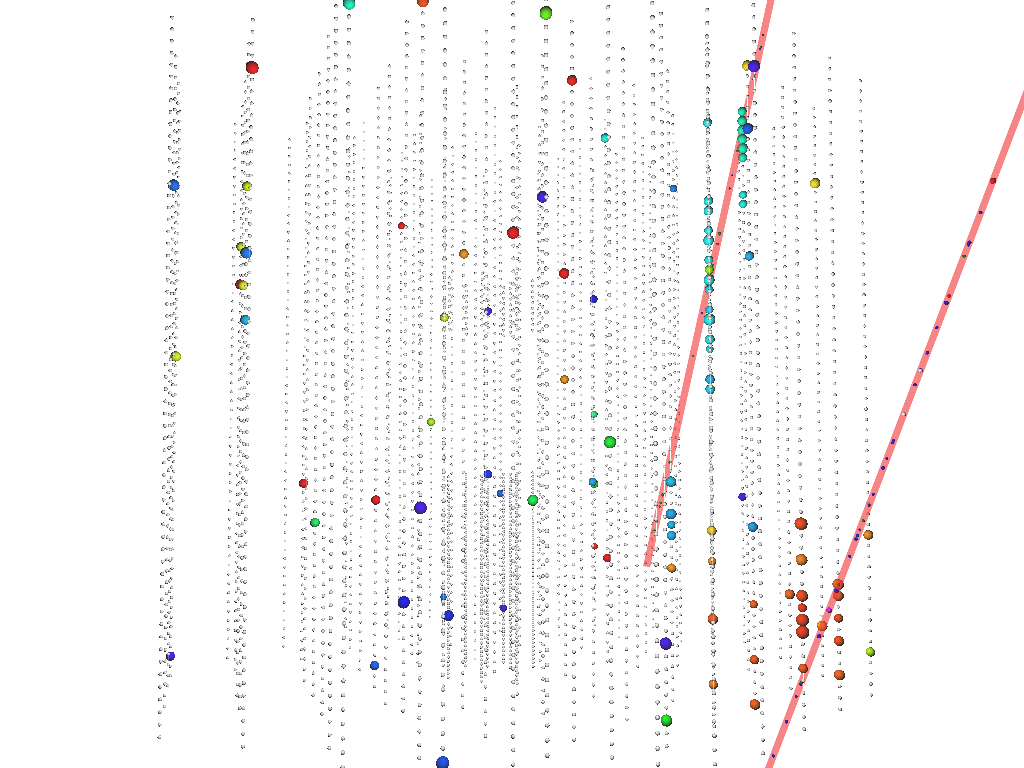
\includegraphics[width=0.8\textwidth]{chapter7/img/coincidenteventsCORS.png}
\caption{Event display of a simulated coincident event of two downgoing muons. The colors of the event range from red (early) to blue (late). The first muon hits the bottom of the detector, while the second traverses mainly the upper part. These events are reconstructed as a single upgoing event and therefore result in a large background contribution for analyses that focus on upgoing tracks such as this one. The scattered isolated hits are due to noise effects and mostly removed by pulse cleaning.}
\label{fig:coincidentevent}
\end{figure}

\noindent There are two modules that try to clean events more thoroughly than pulse cleaning alone. The first is \texttt{TopologicalSplitter}\index{TopologicalSplitter} (TS), which starts from the Q-frames and loops over pulses and splits the event into clusters of pulses that contain at least a number of causally\footnote{The time between two DOM hits cannot be less than the time that light would have taken.} connected pulses within a certain time window. Some extra cleaning, similar to \texttt{seededRT} cleaning, is done in addition and can split coincident events that have overlapping readout windows, but are geometrically separated.

The second module, also used in this analysis, is called \texttt{IceHive}. A full description can be found in the doctoral thesis of M. Zoll \cite{mzollthesis}. The module consists of two main parts: one that splits events and handles coincident events, \texttt{HiveSplitter}, and another that has a refined pulse cleaning, \texttt{HiveCleaning}.

\subsection{\texttt{HiveSplitter}}
The module assumes that individual particles creates \textit{clusters} of hits in the detector. A cluster can grow within a certain time window, but is separated from another cluster if it's not spatially connected. An initial cluster is formed if the multiplicity of hits exceeds a certain threshold (usually 3 or 4). The main difference in this module versus \texttt{TopologicalSplitter} is that it uses hexagons to describe the detector instead of assuming a spherical parameterization. It makes more sense to optimize the search volume, where hits are clustered together, with a shape that describes the detector well and uses a discrete spacing between larger volumes instead of a uniformly growing sphere. The hexagonal shape is set by defining three heights. The first height, $h_1$, is defined along the string of the hit DOM and is equal to the vertical distance along the string. The second height, $h_2$, is the vertical height along the neighboring strings. The third height, $h_3$, is the vertical height along the next-to-neighboring strings. An example is shown in Figure \ref{fig:hexagon} (\textit{left}).

\begin{figure}[t]
\centering
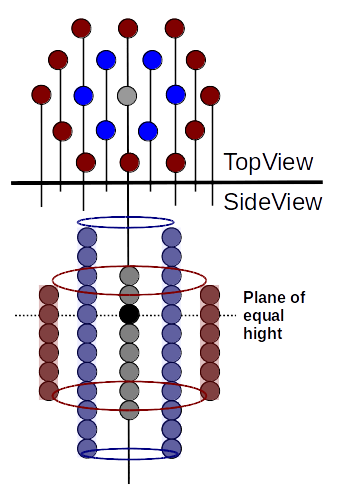
\includegraphics[width=0.5\textwidth]{chapter7/img/hexagons.png}
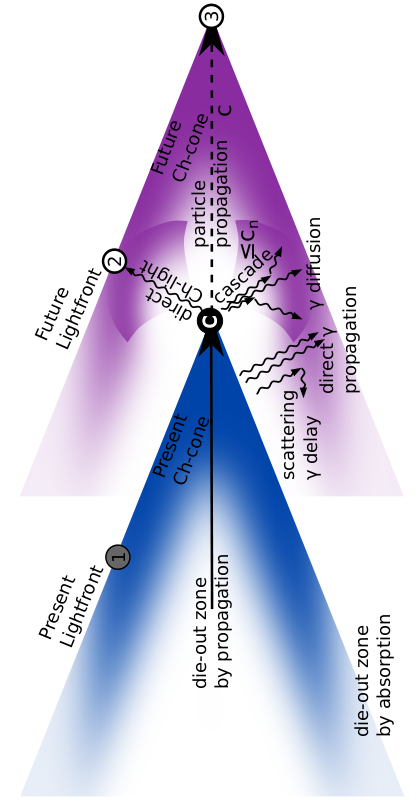
\includegraphics[width=0.4\textwidth]{chapter7/img/cherenkovzoll.png}
\caption{\textit{Left: }The black circle illustrates a DOM that triggered a hit in the detector. The grey circles symbolize the DOMs along the string of the hit DOM. The number of DOMs that can be included in the active volume depends on the heights defined by the module. The blue/purple DOMs belong to the neighboring strings and the red/brown DOMs to the next-to-neighboring strings. The heights of both these sets of DOMs are also set by the module. This example shows $h_2 > h_1 > h_3$, where $h_i$ is the height of the $i$-th string from the center. The heights are asymmetric in this example. \textit{Right: }Illustration of Cherenkov emission profile of a traversing particle. Both figures from Ref. \cite{mzollthesis}.}
\label{fig:hexagon}
\end{figure}
When the active region is set, there is an additional check to see if DOMs can be ``connected''. \texttt{IceHive} assumes certain emission profiles (for both cascades and tracks) where light is produced. Three possible connections are assumed:

\vspace{2mm}
\begin{enumerate}
\item Hits occur at the same time, but at a spatial distance in agreement with the Cherenkov emission profile (hits C\&1 and 2\&3 in Figure \ref{fig:hexagon} (\textit{right})).
\item Hits occur at a different time and a different location, but in agreement with the Cherenkov emission profile (hits C\&2 in Figure \ref{fig:hexagon} (\textit{right})).
\item Hits on topologically identical sites of an emission pattern that has moved along with the propagation of the particle (hits C\&3 and hits 1\&2 on Figure \ref{fig:hexagon} (\textit{right})).
\end{enumerate}
\vspace{2mm}

\noindent These clusters are finally separated into different P-frames. Each P-frame is assumed to originate from a different primary particle.

\subsection{\texttt{HiveCleaning}}
Additionally, a similar cleaning as explained in Section \ref{sec:pulsecleaning} can be performed. Isolated hits that do not have neighboring hits occurring within a certain distance and time window, are removed. The main difference between this and \texttt{seededRT} cleaning is that the module again uses the hexagons as defined in the previous section.\\

\subsection{Remark}
\noindent The use of \texttt{IceHive} has a better performance in separating coincident events compared to \texttt{TopologicalSplitter} (see Ref. \cite{mzollthesis}), but often ``over-performs'' and splits clusters of hits that are originating from the same particle. This is predominantly the case for dim tracks that have large separations in between clusters (most of the triggered SMP events are of this type). To reduce this type of error, the module \texttt{CoincSuite} \index{CoincSuite} was designed, again by M. Zoll \cite{mzollthesis}.

\section{CoincSuite}
\begin{figure}[t]
\centering
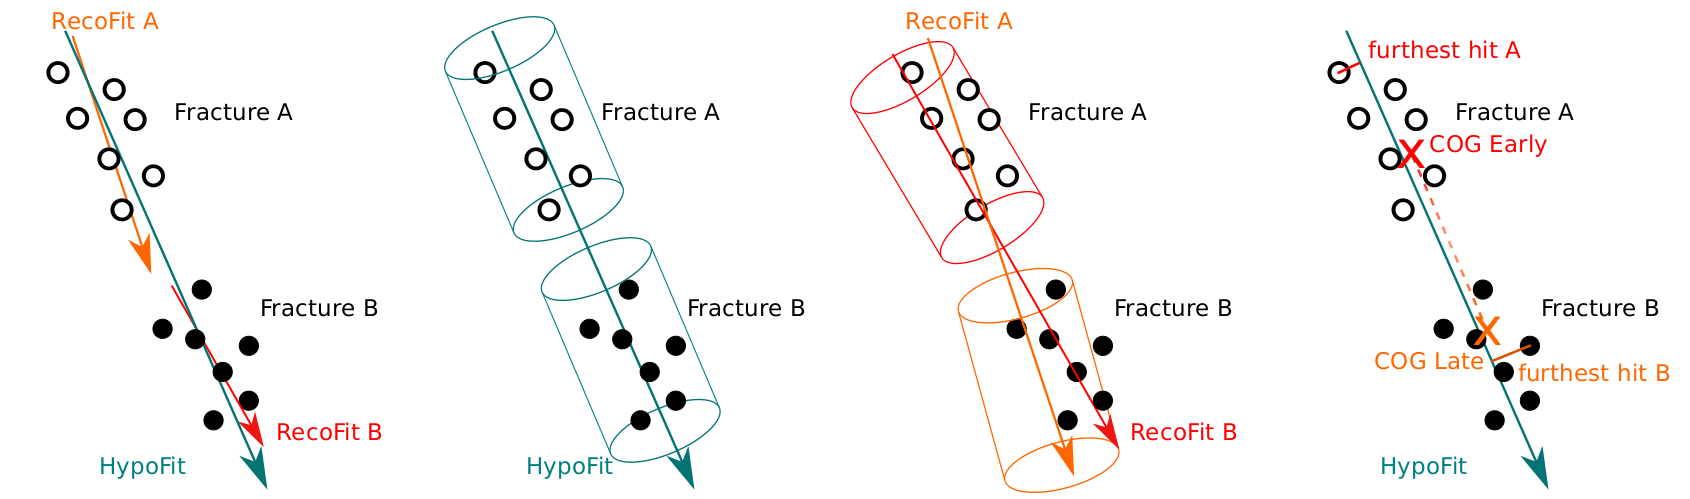
\includegraphics[width=\textwidth]{chapter7/img/coincsuite.png}
\caption{Schematic illustrations of possible recombination scenarios with the \texttt{CoincSuite} module. Two events are compared to each other or the combined event (HypoFit) in several different ways. Figure from Ref. \cite{mzollthesis}.}
\label{fig:coincsuite}
\end{figure}
Several testing algorithms allow to check if two or more split P-frames can originate from a single event. Five different scenarios were tested in this analysis, the first four are also chronologically shown in Figure \ref{fig:coincsuite}:
\vspace{2mm}

\begin{enumerate}
\item Cluster alignment: the reconstructed direction of the individual clusters is compared to the direction of a reconstruction that uses the combined hits (HypoFit). The directions should be within a certain critical angle.
\item Cylinder cluster containment: the DOMs of the individual clusters should be able to be grouped together in a cylinder that has its center and direction along the HypoFit.
\item Cylinder cluster alignment: a cylinder around the reconstruction of each cluster is draw. The cylinders should overlap within a certain fraction.
\item COG\footnote{Similar to COM (Center Of Mass), the COG is a weighted average position of the hit DOMs. DOMs that register more light get a higher weight.}\label{footnote:cog} connection: the COG of the second quarter of hits of the the first cluster and the COG of the third quarter of hits of the second cluster are computed. These COGs should lie close enough and have to be in the vicinity of the HypoFit.
\item Velocity test: tests if the velocity of the HypoFit is close to the speed of light.
\end{enumerate}

\vspace{2mm}
\noindent The combination of \texttt{IceHive} (which does a very good job in cleaning events, but often over-performs and splits events that shouldn't be) and \texttt{CoincSuite} (which recombines events that were wrongfully split), leads to a very powerful tool to clean events.

%\section{Analysis techniques}
%\textcolor{red}{Komt hier iets dat je gebruikt in het volgende hoofdstuk maar nog niet hebt uitgelegd?}

\section{Event cleaning and reconstructions: summary}
The previous sections described how events can be cleaned and how several reconstruction algorithms work. In Chapter \ref{ch:icecube}, we described how such an event is constructed. Several triggers read out series of hits in the IceCube detector within a time window to an event. A hit consists of a DOM pulse, the DOM location and a timestamp. One DOM can have multiple hits in an event.

Reconstruction algorithms try to reconstruct certain particle properties such as the direction, location and track length. Cleaning algorithms remove noise hits and split clusters of hits that originate from coincident events to separate events.\\

\noindent Aside from cleaning and reconstruction, which are done on single events, several analysis techniques are also used in this work. These algorithms look at large samples and try to classify events as signal- or background-like. Therefore, Monte Carlo samples of both signal and background samples are used. The first algorithm that is discussed below is ``minimal-Redundancy-Maximum-Relevance'', which tries to filter out the most powerful variables from a large set of variables. Secondly, we discuss a machine learning technique called ``Boosted Decision Trees''. Such an algorithm is trained with Monte Carlo samples to ``learn'' how to discriminate signal from background events and outputs a single-valued parameterization. This can then be applied to real data.



\section{Minimal-Redundancy-Maximum-Relevance}
\label{sec:mrmr}
Having multiple variables that are able to discriminate signal from background events is a necessary tool that ensures the ability to conclude statements on a certain theory or exotic phenomenon. Single variables can show promising results, but when multiple variables are highly correlated, much of the discriminative power diminishes. When using BDTs, analyzers often try to include variables and remove them if they show to be highly correlated in a trial-and-error fashion.

In this analysis, I made use of a technique that was originally developed for analyses in biological sciences but can be used for most analyses that involve ``data mining''. Variables from a large sample set were selected with the condition of minimal-Redundancy-Maximal-Relevance (mRMR). To optimize the characterization of a certain class of events with a set of variables, these variables are selected with a \textit{maximal relevance}. Here, ``relevance'' is characterized in terms of correlation of mutual information. Because combinations of individually good features do not necessarily lead to good classification performance, there is the additional requirement of \textit{minimal redundancy}. The algorithm sorts variables according to their importance (defined as having a minimal redundancy and maximum relevance). More information about this algorithm can be found in Ref. \cite{1453511}.\\

\noindent In this analysis, mRMR was used to rank variables from a large set according to their importance and proved to lead to low correlated variables (as can be seen in the Appendix in Figure \ref{fig:correlation}).




\section{Boosted Decision Tree classifiers}
\label{sec:BDT}
Given a set of events that have a fixed set of variables constructed in an analysis, the question remains if the event is in fact a \textit{signal} (dim track from an SMP) or \textit{background} (e.g. a muon from $\nu_\mu$ or air showers) event. One can rely on Monte Carlo simulations to get a handle on the variable distribution in both sets. The most general, and still widely used, method is to use a cut-and-count approach where a cut is placed on a certain variable that discards events that fail the requirement. A Boosted Decision Tree (BDT), however, inspects a set of variables by looking at large sample sets that are classified as either signal or background. The BDT is ``trained'' to classify an event to signal-like or background-like. This is done with a ``BDT score'' that ranges from -1 to 1. The higher the score, the more an event is regarded as signal-like. How this is done is given in more detail below. Boosted decision trees rely on multiple individual trees, collectively called a \textit{forest}. Therefore, we will first explain how a single tree classification works.


\subsection{Structure}
The goal of a decision tree is to determine if an event is signal- or background-like. It uses a tree-like structure where certain selection criteria are used at different nodes as illustrated in Figure \ref{fig:bdt}.

\begin{figure}[t]
\centering
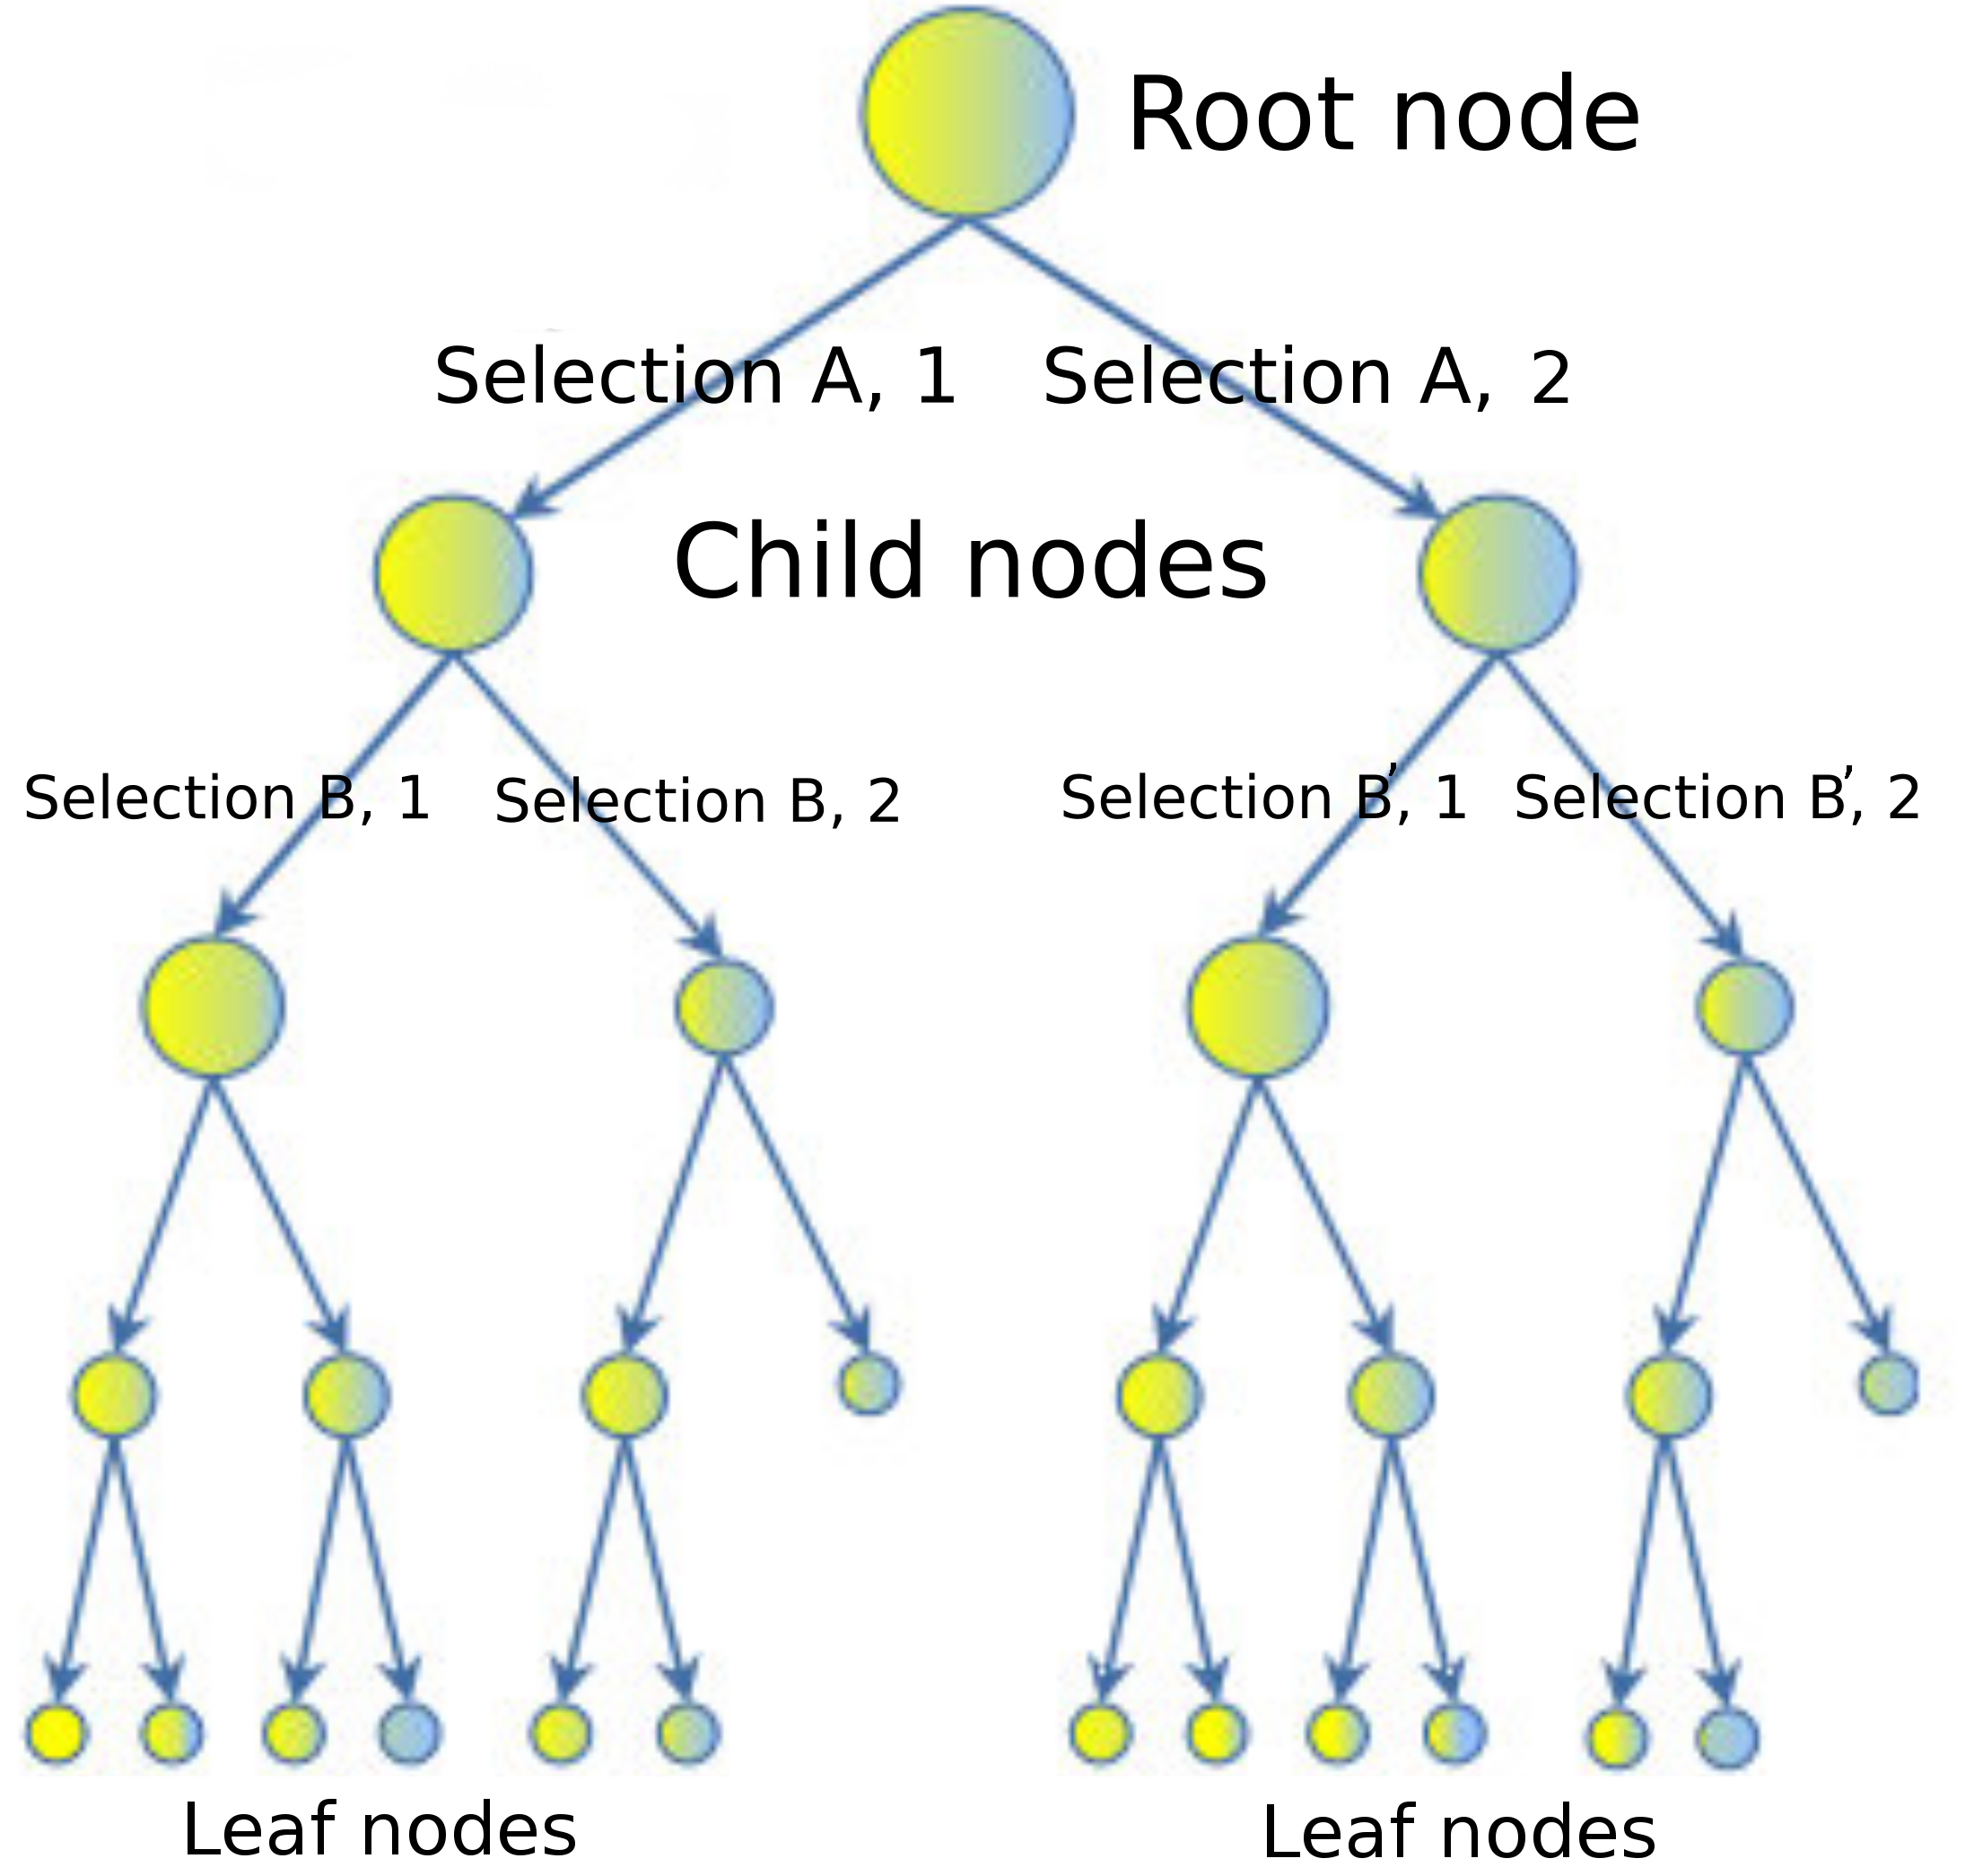
\includegraphics[width=0.5\textwidth]{chapter7/img/bdt.png}
\caption{Illustration of decision tree scheme. Selection B and B' denote a selection on the same variable, but other requirement.}
\label{fig:bdt}
\end{figure}
A decision tree is a binary tree that places an event into a certain node depending on the selection at a node. The depth of a decision tree can be arbitrarily long, but is determined by a set of criteria as defined in Section \ref{subsec:training}. An event consists of a certain set of variables $X = {x_1,x_2,...,x_n}$ that are used in the classification. Before any selection criteria, the event is said to be represented by the \textit{root node}. A binary selection then determines to which \textit{child node} the event should be classified, for example: 

\begin{equation}
\begin{split}
\textrm{Selection A} &= x_1 > y_1 \ \ (\textrm{option 1})\\
&= x_1 \leq y_1 \ \ (\textrm{option 2}),
\end{split}
\end{equation}
where $y_1$ is the cut value for variable $x_1$. Similarly, the other selections determine where the event is eventually placed. The last nodes are referred to as \textit{leaf nodes} and hold the probabilities of whether an event is more signal- or background-like. These probabilities are translated into a score ranging between -1 (background) and +1 (signal). 

\subsection{Training}
\label{subsec:training}
To construct a decision tree, one first has to ``train'' the algorithm on MC. Given a certain ``signal set'' and ``background set'', all variables used in the BDT are histogrammed and at each bin for each variable the ``best cut'' is set at the first node selection. To determine the optimal cut, we first define the purity of a node, $p$, by

\begin{equation}
p = \frac{\sum_s w_s}{\sum_s w_s + \sum_b w_b},
\end{equation}
\noindent where $w_s$ and $w_b$ refer to the weights of the signal and background events\footnote{These are the weights after scaling events to a certain spectrum.}. The Gini index, g,

\begin{equation}
g(p) = p(1-p), 
\end{equation}
is used as a separation variable in this work\footnote{Other possible separation variables include the cross entropy $-p \cdot \ln(p)-(1-p) \cdot \ln(1-p)$ or the misclassification error $1-\textrm{max}(p,1-p)$.}. Using the Gini index, the separation gain determines the effectiveness of the cut

\begin{equation}
\label{eq:separationgain}
\Delta S = g_p \cdot \sum w_p - \left(g_l \cdot \sum w_l + g_r \cdot \sum w_r\right),
\end{equation}
\noindent where $g_p$ and $w_p$ denote the Gini index and weights of the parent nodes and similarly for the left and right child nodes. The cut that gives the highest separation gain is subsequently selected. The algorithm stops when one of the following criteria is met:
\vspace{2mm}

\begin{itemize}
\item a node only consists of signal or background events;
\item a certain predefined maximal depth is reached;
\item splitting would cause a child node to have less than a predefined minimal amount of events left;  
\end{itemize}
\vspace{2mm}
and therefore determines the size of a tree. These selection criteria are necessary to avoid overtraining (see Section \ref{subsec:overtraining}). An example of a very simple decision tree is given in Appendix \ref{ch:adaboostappendix}.


\subsection{Boosting}
\label{subsec:boosting}
As already implied in the text above, a BDT consists of a \textit{forest} of decision trees. A user specified number of individual decision trees are trained sequentially, with a boosting process in between each training. Boosting consists of adjusting the weights of individual events according to whether the previously trained tree classifies them correctly. In this work, the AdaBoost\footnote{Short for Adaptive Boosting.} algorithm was used for boosting in which the score of an event is a weighted average of the scores the event receives from each tree in the forest \cite{FREUND1997119}.

A BDT stands for ``boosted decision tree'', but it must be understood that there are actually many trees (typically hundreds), and that boosting is a process that occurs between the training of consecutive trees. The approach makes use of the power of numbers: many weak single decision trees combined can be more powerful than one very good decision tree. In general, boosting follows the following steps:
\vspace{2mm}

\begin{enumerate}
\item Train a weak model on training data.
\item Compute the error of the model on each training example.
\item Give higher importance to examples on which the model made mistakes.
\item Re-train the model using ``importance weighted'' training examples.
\item Go back to step 2.
\end{enumerate}
\vspace{2mm}
A simple example of a BDT is given in Appendix \ref{ch:adaboostappendix}.\\
\newline
\noindent We define a function to indicate whether an event is classified incorrectly: $I(s,y)=0$ if $s=y$ and $1$ otherwise. The error rate for a tree is then equal to

\begin{equation}
\epsilon = \frac{\sum_i w_i I(s,y)}{\sum_i w_i}.
\end{equation}
\noindent The boosting factor for the tree is defined as

\begin{equation}
\label{eq:boostfactor}
\alpha = \beta \cdot \ln\left(\frac{1-\epsilon}{\epsilon}\right),
\end{equation}
\noindent with $\beta$ a user defined \textit{boosting beta} and changes the weight of the tree to

\begin{equation}
\begin{split}
w' = w \cdot \exp(\alpha), \ \ \ \ \ \ \ \ \ \ \ \ \ \ \ \ \ \ \ \ \ w' = w \cdot \exp(-\alpha)\\
\textrm{ (correct classification)} \ \ \ \ \textrm{ (incorrect classification),}
\end{split}
\end{equation}
\noindent after which the weights are renormalized so that $\sum w' = 1$. The process is repeated until the number of predefined trees is reached.

Due to its definition, the boost factor $\alpha$ will give good classifiers (which have low error rates) large boost values. Events that are misclassified are then given larger weights, making the algorithm more likely to classify them correctly in the subsequent tree classifier.

Once the entire BDT is trained, the events can be given a score based on the multiple tree classifiers. This is done by taking the weighted average of all the scores in the individual tree classifiers, using its boost factor $\alpha$ as the weight of the tree. The score of an event $i$ is then given by

\begin{equation}
s_i = \frac{\sum_m \alpha_m \cdot s_{i,m}}{\sum \alpha_m},
\end{equation}
\noindent where we loop over the individual trees denoted with index $m$.

\subsection{Overtraining}
\label{subsec:overtraining}
BDTs are very powerful tools, but if not used correctly, could lead to problems that are not easy to spot at first sight. Assume we train our BDT with a certain signal set and background set. If the BDT is trained up to the point of classifying statistical fluctuations, there is said to be \textit{training sample overtraining}. An illustrative example is given in Figure \ref{fig:overtrainingexplained}. Another example is data/MC overtraining. The former can be dealt with with the use of \textit{pruning}, while the latter should show clear data/MC disagreement, which is checked in the analysis. 

\begin{figure}[t]
\centering
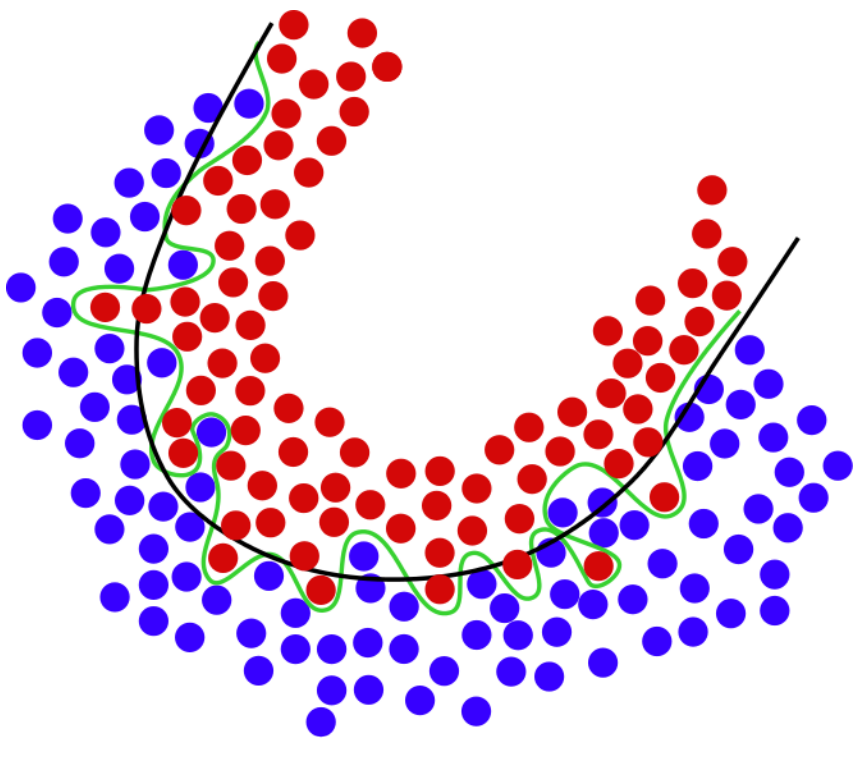
\includegraphics[width=0.5\textwidth]{chapter7/img/overtraining.png}
\caption{Example of overtraining. In black, the theoretical line between background (blue points) and signal (red points) is given. An overtrained BDT will have a (perfect) selection such as the green line. Illustration from \cite{boserpdf}.}
\label{fig:overtrainingexplained}
\end{figure}

\subsubsection{Pruning}
\label{subsub:pruning}
The problem with overtraining is essentially that there are certain splits in a classifier tree that are too specific and less important. In the method of \textit{cost complexity pruning}, for each node the complexity is calculated as

\begin{equation}
\rho = \frac{\Delta S}{n_{\textrm{leaves}} -1},
\end{equation}
\noindent with $\Delta S$ the separation gain as defined in Eq. \ref{eq:separationgain} and $n_\textrm{leaves}$ the number of leaves below the split node. The subtree of the node with the smallest value of $\rho$ is removed and this is done repeatedly until a desired \textit{pruning strength}\footnote{A parameter on a scale from 0 to 100, which specifies the percentage of the pruning sequence to actually execute. 0 means no pruning is done and 100 signifies only a single root node remaining.} is reached.\\
\newline
\subsubsection{Additional checks}
\noindent BDTs are always trained and tested with different subsets of the same type (background or signal) of event. If the training set has significantly different scores than the testing set, the sample is most probably overtrained and one has to change the BDT input parameters. Additional to pruning, one typically uses Kolmogorov-Smirnov testing to indicate if the BDT score distributions from the training and testing sets could follow the same distribution pattern. Therefore, a $p$-value equal to the statistical probability that two samples are drawn from the same distribution is computed. Because training and testing samples will never be identical, there will always be some level of overtraining. As a rule of thumb, a $p_{KS} \lesssim 0.01$ indicates overtraining beyond the level of comfort. Appendix \ref{ch:bdtchecks} shows the result of such checks.
	

